% ---------------------------------------------------------------------------
% Author guideline and sample document for EG publication using LaTeX2e input
% D.Fellner, v1.13, Nov 13, 2007

\documentclass{egpubl}

% --- for  Annual CONFERENCE
\VisualComputing % VisualComputing (added by U. Schwanecke, 2021)
%\ThreeDAnimation % 3DAnimation (added by U. Schwanecke, 2020)
%\Seminar % Specialist Seminar (added by U. Schwanecke, 2019)
%\ConferenceSubmission % uncomment for Conference submission
%\ConferencePaper      % uncomment for (final) Conference Paper
%\STAR                 % uncomment for STAR contribution
% \Tutorial             % uncomment for Tutorial contribution
% \ShortPresentation    % uncomment for (final) Short Conference Presentation
%
% --- for  CGF Journal
% \JournalSubmission    % uncomment for submission to Computer Graphics Forum
% \JournalPaper         % uncomment for final version of Journal Paper
%
% --- for  CGF Journal: special issue
% \SpecialIssueSubmission    % uncomment for submission to Computer Graphics Forum, special issue
% \SpecialIssuePaper         % uncomment for final version of Journal Paper, special issue
%
% --- for  EG Workshop Proceedings
% \WsSubmission    % uncomment for submission to EG Workshop
% \WsPaper         % uncomment for final version of EG Workshop contribution
%
%\electronicVersion % can be used both for the printed and electronic version

% !! *please* don't change anything above
% !! unless you REALLY know what you are doing
% ------------------------------------------------------------------------

\PrintedOrElectronic

\usepackage[pdftex]{graphicx} 
\usepackage{t1enc, dfadobe}
%\usepackage[T1]{fontenc}
\usepackage{egweblnk}
\usepackage{cite}

% For backwards compatibility to old LaTeX type font selection.
% Uncomment if your document adheres to LaTeX2e recommendations.
% \let\rm=\rmfamily    \let\sf=\sffamily    \let\tt=\ttfamily
% \let\it=\itshape     \let\sl=\slshape     \let\sc=\scshape
% \let\bf=\bfseries

% end of prologue

\usepackage{blindtext}
\usepackage{caption}
\usepackage{subfigure}
\usepackage{dblfloatfix}
\usepackage{adjustbox}
\usepackage{mathtools}
\usepackage{todonotes}

\usepackage{cleveref}


% ---------------------------------------------------------------------
\captionsetup{labelfont=bf,textfont=it}
\title[Burst Images]%
      {Burst Images}

\author[Sascha Scheid]
    {\parbox{\textwidth}
        {\centering 
			Sascha Scheid
        }
        \\
    {\parbox{\textwidth}
        {\centering RheinMain University of Applied Sciences, Wiesbaden, Germany\\
       }
    }
}
% ------------------------------------------------------------------------

% if the Editors-in-Chief have given you the data, you may uncomment
% the following five lines and insert it here
%
% \volume{36}   % the volume in which the issue will be published;
% \issue{1}     % the issue number of the publication
% \pStartPage{1}      % set starting page


%-------------------------------------------------------------------------
\begin{document}

%-------------------------------------------------------------------------
% uncomment for using teaser (comment if you don't want a teaser)
\teaser{
    \hspace{\fill}
    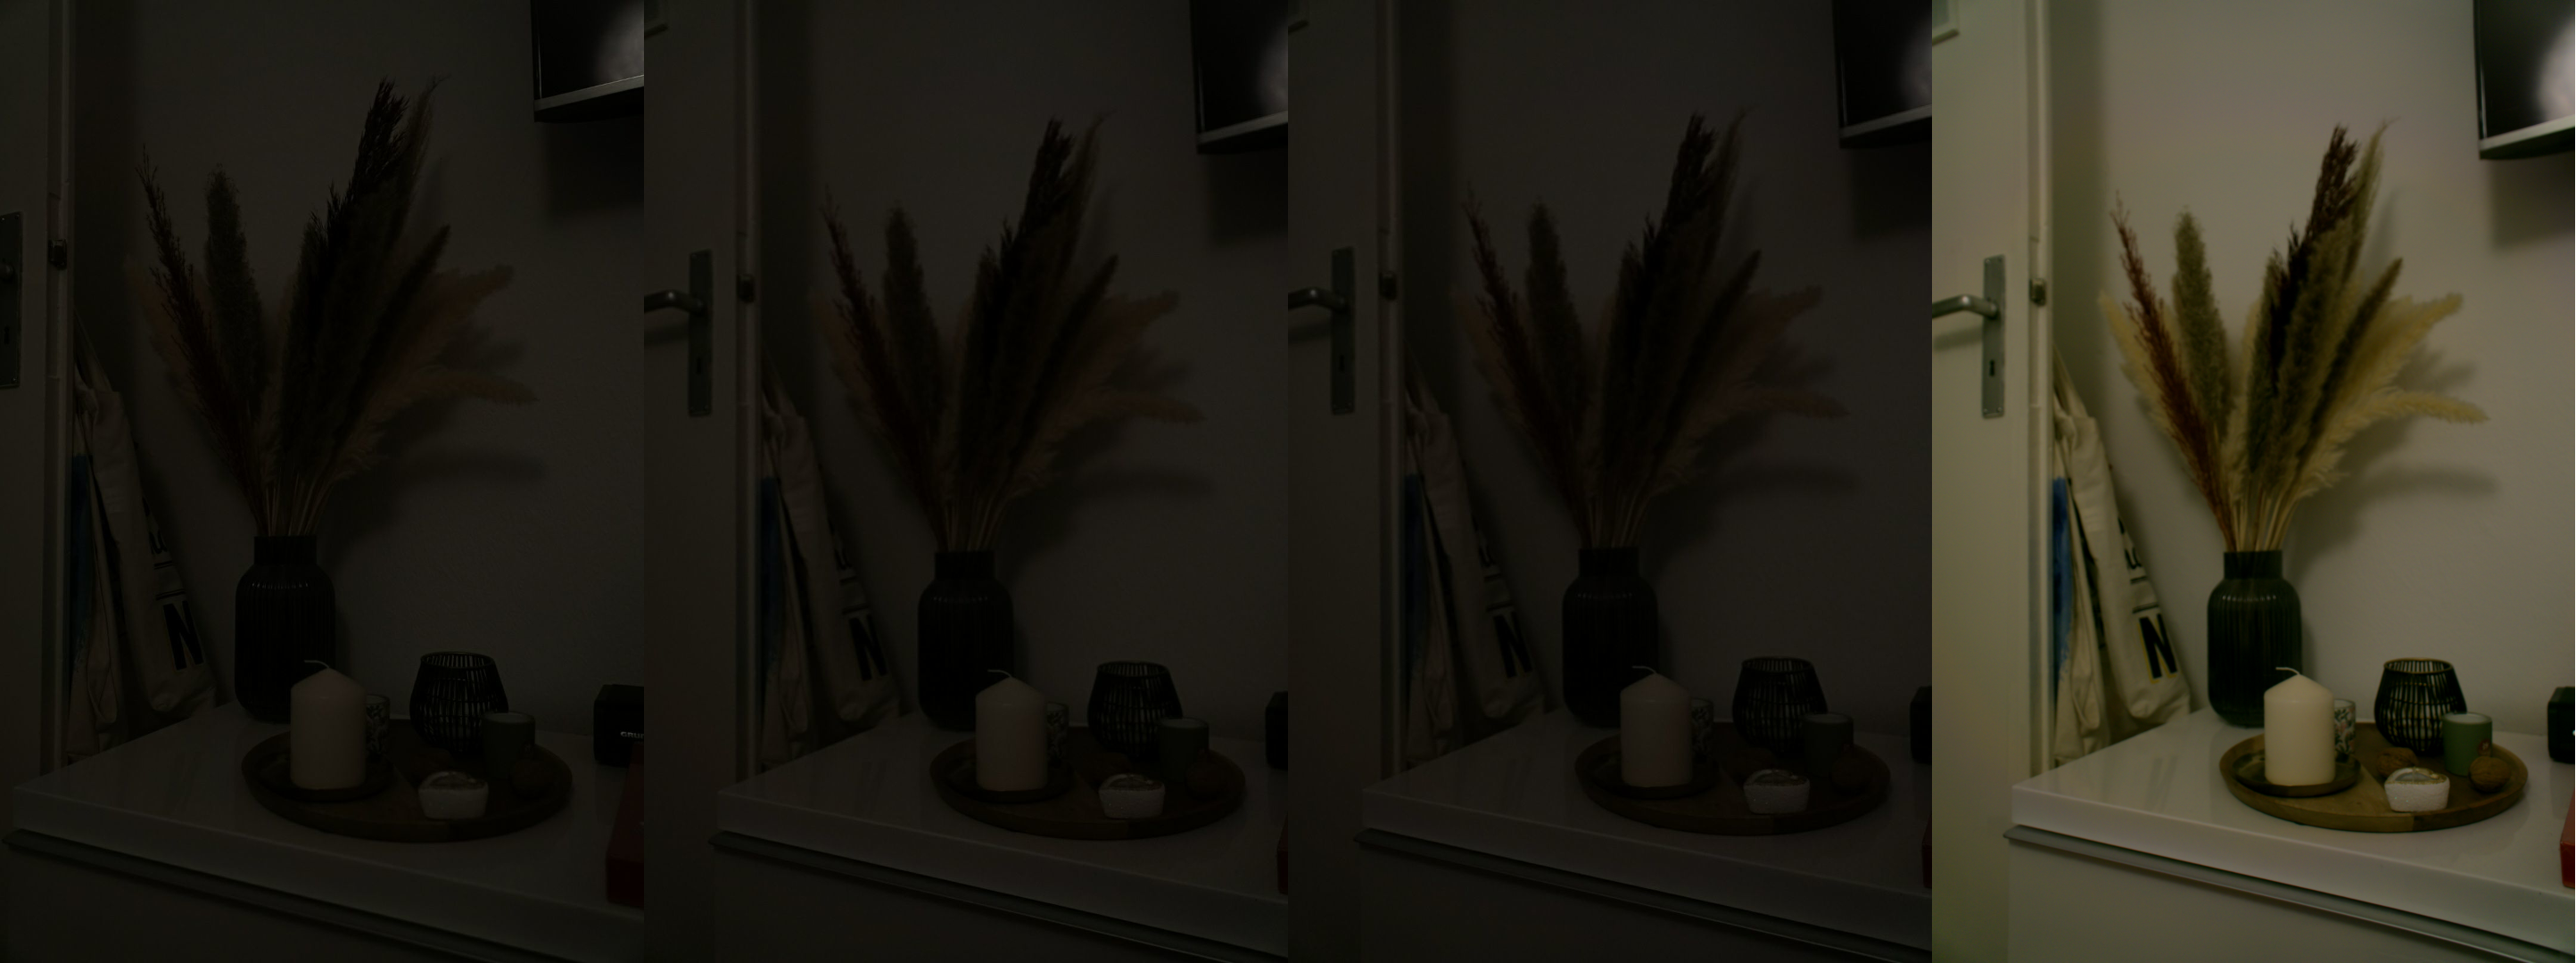
\includegraphics[width=0.9\linewidth]{images/teaser.png}
    \hspace{\fill}
    \centering
    \caption{
      Left images: Sample from a image burst captured with a Sony Alpha A6000 camera
                   with focal length $18mm$, shutter speed $1/50s$, ISO $400$ 
                   and aperture $f/4.0$ in a low light situation.
      Right image: Processed image burst with settings gain $g = 1.2$ and dynamic 
                   range compression $c = 3.0$.
    }
    \label{fig:teaser}
}


%-------------------------------------------------------------------------
\maketitle


%-------------------------------------------------------------------------
\begin{abstract}
Compared to cameras built specifically for photography, cameras used in smartphones 
suffer from constructional limitations that restrict image quality, such as smaller 
sensors and pixels, shorter focal lengths and smaller apertures. To compensate for 
these limitations, techniques from computational photography are used, whereby many 
current improvements are based on the processing of several similar images of the same 
scene - so-called image bursts. In the course of this work, an existing implementation 
of a burst processing pipeline was examined more closely and applied to example bursts 
from mobile and DSLR cameras. In order to enable as many people as possible to 
experiment with this implementation, it was adapted in such a way that it can be 
used platform-independently. Even if performance and operation are not sufficient 
to be used in a business context, it is suitable for an introduction to and initial 
experimentation with burst processing.
\end{abstract}  


%-------------------------------------------------------------------------
\section{Introduction}
\label{sec:introduction}

Burst photography is a technique in which a series of photographs is taken quickly in succession.
This can be useful in a variety of situations, such as capturing action or movement, 
or to create a sense of motion. In digital photography, burst images are stored as a 
sequence of image files, typically in a format such as JPEG or RAW.

High Dynamic Range (HDR) is a technique used to improve the dynamic range of an image, 
which is the range of luminance or brightness levels that can be captured in a photograph. 
The dynamic range of a scene can often be greater than what a camera is able to capture 
in a single image, resulting in lost detail in the highlights or shadows. 
HDR techniques can be used to extend the range of luminance in an image, 
resulting in more detail and a more realistic representation of the scene.

One way that burst photography and HDR techniques can be used together
is to capture a series of photographs with different exposures in a burst, and then combine 
the exposures into a single HDR image using software. This technique is known as 
\textit{exposure bracketing} and is described by Mann {\&} Picard (2019) \cite{mann1994bracketing}. 
This can be particularly useful in low-light situations, where the camera may struggle to 
capture a wide range of luminance levels in a single exposure. By capturing multiple exposures and combining them into an 
HDR image, it is possible to extend the dynamic range and capture more detail in both the 
highlights and shadows.

According to the photo sharing community Flickr, the most 
popular cameras among users are those built into mobile phones \cite{flickr2023popularity}. Unlike dedicated photo cameras, these have 
some inherent disadvantages which are outlined by Delbracio et al. (2021) \cite{delbracio2021mobile}. 
They include:

\begin{itemize}
    \item Low sensitivity: Mobile cameras often have smaller sensors compared 
          to DSLR or mirrorless cameras, which can result in lower sensitivity 
          to light. This can make it difficult to capture usable images in low l
          ight conditions without using long exposures or high ISO values, 
          which can introduce noise and other artifacts.

    \item Limited zooming capability: Due to its small form factor, it is difficult to mount a lens 
          with a highly variable focal length in front of the sensor of a cell phone.
          Thus, they have to heavily rely on digital zoom instead of optical zoom which can lead to loss 
          in sharpness of the zoomed in image.
    
    \item Limited dynamic range: Mobile cameras can have limited dynamic range, 
          which can make it difficult to capture both the shadow and highlight 
          details in a scene. This can result in underexposed or overexposed 
          areas in the image, and can be particularly challenging in low light 
          conditions where the range of luminance values is often greater.
    
    \item Motion blur: Long exposures are often necessary in low light conditions, 
          which can result in motion blur if the camera or the subject is moving. 
          This can be particularly problematic for handheld shots or when photographing 
          moving subjects.
\end{itemize}

To address these constraints, several techniques can be used to improve the performance 
of mobile cameras in low light conditions. These include:

\begin{itemize}
    \item Noise reduction: Noise reduction algorithms can be used to reduce the noise 
          introduced by high ISO values or long exposures. These algorithms can smooth 
          out the image while preserving edges and other important details.

    \item High dynamic range techniques: HDR techniques, such as burst photography 
          and computational photography, can be used to extend the dynamic range of mobile 
          cameras and capture more detail in both the shadow and highlight areas of an image.
    
    \item Image stabilization: Image stabilization technologies, such as optical image 
          stabilization or electronic image stabilization, can be used to reduce the 
          effects of camera shake or subject movement during long exposures.
\end{itemize}

While there are still limitations to the capabilities of mobile cameras compared to larger, 
more specialized cameras, advances in technology and image processing algorithms are 
continually improving the quality and performance of mobile cameras in a variety of 
lighting conditions.


%-------------------------------------------------------------------------
\section{Related Work}
\label{sec:related_work}

The HDR+ image processing pipeline is a computational photography technique developed by Google for use 
in the Google Pixel smartphone. It is designed to capture high dynamic range images using 
burst photography. The algorithm uses computational techniques to extend the dynamic range 
of the captured images, rather than relying on multiple exposures as in traditional 
HDR techniques, in which a rapid sequence of images at different exposures is captured.
The captured images are merged to create a single HDR image. The HDR+ algorithm was developed 
to improve the quality and dynamic range of images captured on mobile devices, particularly in 
low-light conditions. The HDR+ algorithm consists of several steps, which are outlined in detail 
by Hasinoff et al. (2016) \cite{Hasinoff2016burst}. In brief, the steps are as follows:

\begin{enumerate}
    \item Burst capture: A sequence of raw images is captured. In contrast to the classic 
          multi-exposure approach, each image will be underexposed and all images have the
          same exposure. An image burst consists of two to eight single images.
    \item Image alignment: The sharpest image of the first three images in the burst is 
          selected as reference image and the remaining images in the burst are aligned 
          to it. This corrects for any movement or misalignment between frames.
    \item Image merging: The aligned raw images are merged to create a single intermediate 
          raw image that will then be further processed.
    \item Finishing: The merged image undergoes a set of operations including general
          correction, demosaicking and tone mapping. The most important operation is
          dynamic range compression which reduces the contrast between light and dark
          areas while preserving local contrast. To do so, the local tone mapping method
          \textit{exposure fusion} described by Mertens et al. (2007) \cite{mertens2007exposure} 
          was used, which blends together the best parts of differently exposed images. 
          As there is only one merged image left after step 3, the ones to blend are created synthetically 
          from the merged image.
\end{enumerate}

To increase the amount of light collected, Levoy {\&} Pritch (2018) \cite{levoy2018psl} describe 
the positive shutter lag recording technique, which, unlike zero shutter lag, does not 
continuously capture frames of the scene in a ring buffer, but only after the shutter button is pressed,
which allows longer exposures of the scene. However, this recording technique is more susceptible to motion blur.
This problem was addressed by Liba et al. (2019) \cite{liba2019handheld} who further improved the HDR+ 
pipeline by collecting real-time motion data before the shutter button is pressed. Based on this data, the motion 
during the shot is predicted and an appropriate exposure duration is selected. In addition, 
they use a learning-based approach for auto-white balancing, which has been specially trained 
for night situations.

Wronski et al. (2019) \cite{Wronski2019superres} describe a super-resolution based image processing pipeline that 
is based on burst image processing pipelines like HDR+. It utilizes the inherent micro movement of hands while
taking pictures with a mobile device to capture multiple frames of a scene with minimal offsets. Unlike other
image processing pipelines, their approach does not include explicit demosaicking.

An approach to image burst processing based only on neural networks was developed by Dudhane et al. (2022)
\cite{Dudhane2022restoration}. They create a set of synthetic burst features by combining information of the
captured images and afterwards merge them in multiple steps while increasing resolution continuously. 

%-------------------------------------------------------------------------
\section{Approach}
\label{sec:approach}

To check how the HDR+ image processing pipeline described by Hasinoff et al. (2016) \cite{Hasinoff2016burst}
handles scenes under different lighting
conditions, an implementation of the pipeline should be made to work and applied to
different image bursts. The implementation used was developed by Timothy Brooks
\cite{Brooks2016git} and published as open source project.

\subsection{Difficulties in getting the project to work}
\label{sec:difficulties}

Unfortunately, the project did neither compile out of the box 
nor was it well documented because it was not maintained for quite some time, so I 
needed to research which dependencies are needed to compile it.

It was documented that the implementation uses Halide \cite{halide2022}, which is a programming language
embedded in C++ that provides a higher level API to efficiently manipulate images. Halide
itself relies on LLVM \cite{llvm2022}. But the project does not compile with the current version
of Halide, which is version 14 at the time of writing. There was a git commit message
that explicitly mentions Halide version 10. Halide version 10 itself did not compile with
the current version of LLVM, which is version 14 at the time of writing. Instead it needs
LLVM version 10. Unfortunately, the operating system I was using, Ubuntu 22.10 \cite{ubuntu2022}, 
does not have that LLVM version in its package repository so I had to compile it myself, which took
quite some time. 

\subsection{Making the project platform independent}
\label{sec:resolving}

Since it is not user-friendly to compile the project and all its dependencies by hand and thus it 
is also difficult to write a universal manual for different operating systems, the idea came up to 
make it platform independent by means of containerization. Docker was chosen as the containerization 
technology because of its prevalence and acceptance. 

In a multi-step build process, a Docker image based on Ubuntu 20.10. is created that contains the 
executable HDR+ implementation and runs it on container startup. The resulting Docker image is 
456 MB in size and can be made available via image registries without users having to compile themselves.

\subsection{Processing multiple bursts in parallel}
\label{sec:parallel}

Since the implementation is designed to process only one image burst, there is a large overhead 
due to the necessary starting and stopping of a container. To address this issue, a shell script 
was created that starts an image processing pipeline for each image burst in a bursts directory 
shared between the operating system and the container when the container is started. Since the 
implementation accepts start parameters to adjust the amount of gain and dynamic range compressen 
applied when processing a burst, these can be set in a configuration 
file for the burst. \Cref{fig:architecture} illustrates the architecture described beforehand. 
The start parameters as well as the output of the processing pipeline are saved 
in a log file, which is stored in the respective burst directory just like the result image.
To avoid reprocessing the same image burst over and over again, all individual burst folders containing 
a result image with default name are excluded from processing. 

\begin{figure}
    \hspace{\fill}
    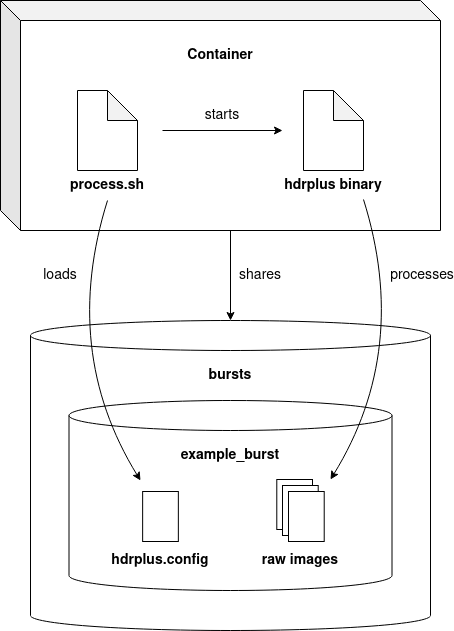
\includegraphics[width=0.9\linewidth]{images/architecture.png}
    \hspace{\fill}
    \centering
    \caption{Architecture of the dockerized application}
    \label{fig:architecture}
\end{figure}

%-------------------------------------------------------------------------
\section{Experiments}
\label{sec:experiments}

To check how reliably the HDR+ implementation delivers good results, 
several image bursts from different scenes were processed. The results 
are presented in the following sections.

\subsection{Low light situations}
\label{lowlight}

As a first test of the pipeline, several images of a dried flower 
were taken in a poorly lit room in the evening. To get even darker 
raw images, shutter speed and ISO were intentionally set lower than 
would be appropriate for the lighting situation. After the burst was
processed by the HDR+ implementation, a pleasing result came out. 
In \Cref{fig:teaser}, an excerpt of the burst is compared to the result.


\subsection{Images with high noise}
\label{sec:noise}

\begin{figure}
      \hspace{\fill}
      \includegraphics[width=0.9\linewidth]{images/noise.png}
      \hspace{\fill}
      \centering
      \caption{
            Left images: Noisy low light sample from bursts provided by the supplemental dataset
            to \cite{Hasinoff2016burst}. Top row shows full image while bottom shows zoom in noisy
            area.
            Right images: Processed burst images with settings gain $g=1.0$ and dynamic 
            range compression $c=2.5$.
      }
      \label{fig:noise}
\end{figure}

To check how well the HDR+ implementation is able to handle image bursts that have high noise, several 
images were processed. The scenes that were checked show objects and people inside enclosed 
spaces as well as a city at night. As can be seen in \Cref{fig:noise}, the noise was 
removed very well in all examples. Even when zooming in, hardly any noise is visible 
compared to the original image. The results were all obtained using same starting 
parameters gain $g=1.0$ and dynamic range compression $c=2.5$ and were satisfactory throughout.



\subsection{Low contrast or dynamic range situations}
\label{sec:contrast}

\begin{figure}
      \hspace{\fill}
      \includegraphics[width=0.9\linewidth]{images/contrast_burst.png}
      \hspace{\fill}
      \centering
      \caption{
            Left images: Low contrast sample from bursts provided by the supplemental dataset
            to \cite{Hasinoff2016burst}.
            Right images: Processed burst images with settings gain g and dynamic 
            range compression c from top to bottom image: $g=1.0$, $c=2.5$ | $g=1.0$, $c=1.5$ | $g=1.0$, $c=1.5$.
      }
      \label{fig:contrast}
\end{figure}

Various image bursts were processed where the raw images were very pale 
and low in contrast. After processing, good results were obtained, showing 
a high dynamic range. \Cref{fig:contrast} compares a sample image from the image burst 
with the processed result, showing the difference in dynamic range. While 
increasing the dynamic range is basically well possible, individual parameters 
per image have to be tried out here compared to the experiments in \cref{sec:noise}, 
which depend on the respective lighting situation. Thus, a too high gain 
parameter can quickly lead to an overexposed and a too high dynamic range 
compression parameter to a comic-like looking result image.

\subsection{Moving objects}
\label{sec:moving}

\begin{figure*}
      \hspace{\fill}
      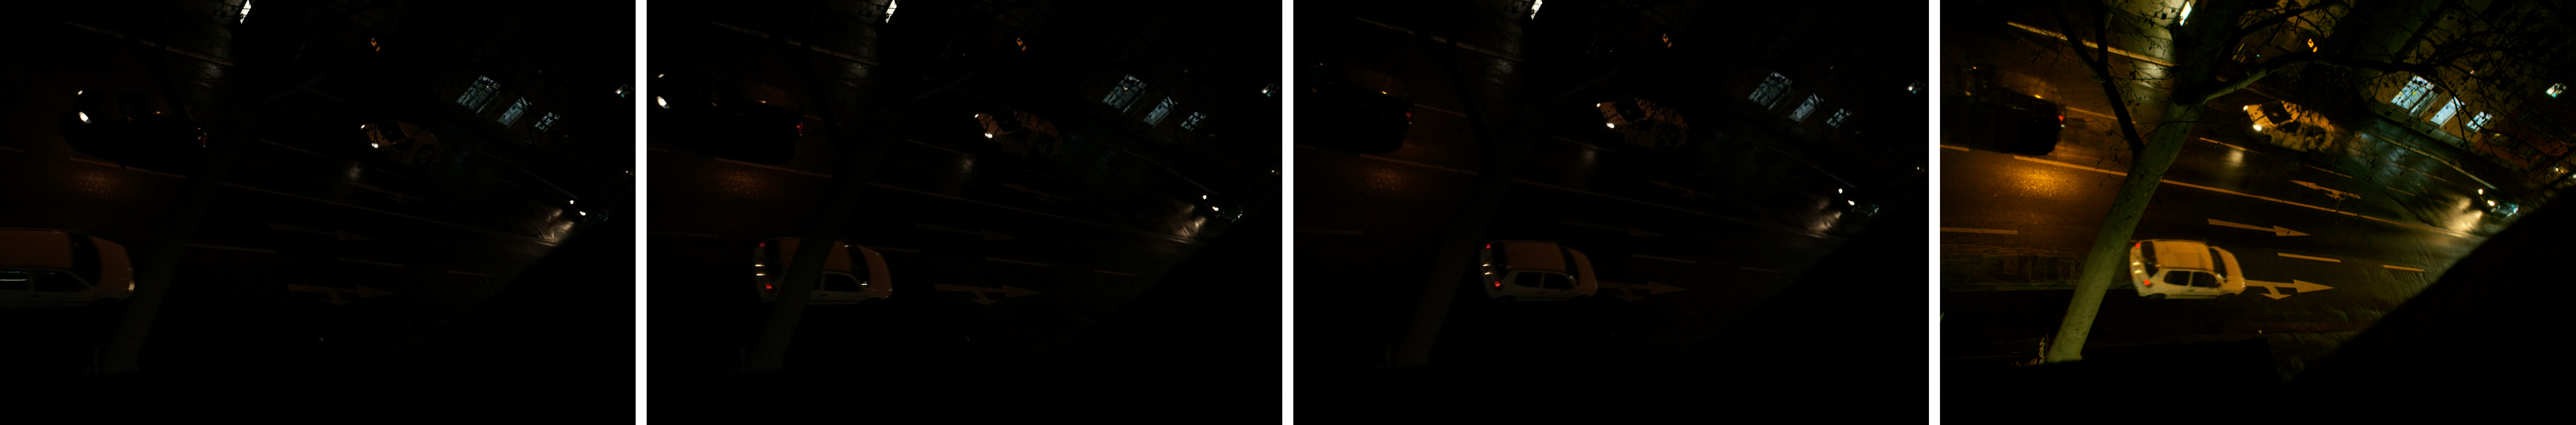
\includegraphics[width=0.9\linewidth]{images/moving_burst.png}
      \hspace{\fill}
      \centering
      \caption{
            Left images: Sample from a image burst captured with a Sony Alpha A6000 camera
            with focal length $18mm$, shutter speed $1/100s$, ISO $680$ 
            and aperture $f/4.0$ in a low light situation with moving cars.
            Right image: Processed image burst with settings gain $g = 1.6$ and dynamic 
            range compression $c = 3.0$. Ghosting is clearly visible when looking at the 
            fast moving white car in the bottom but not when looking at the slower cars
            in the top.
      }
      \label{fig:moving}
\end{figure*}

While small movements could be processed well, it should be investigated how to 
process fast moving objects over a long distance. For this purpose, an image burst 
of a road with moving cars at night was recorded, which is shown in \cref{fig:moving}. 
Although the low light situation was basically processed satisfactorily and not 
too fast cars could be aligned well, clear ghosting artifacts can be seen in the 
for the very fast moving white car.

%-------------------------------------------------------------------------
\section{Conclusions}
\label{sec:conclusion}

By containerizing Brooks' \cite{Brooks2016git} open source project, it is possible 
to process multiple raw image bursts simultaneously with the HDR+ 
image processing pipeline, independent of the host operating system. Users no 
longer need to compile the application themselves and worry about dependencies, 
but could simply pull the Docker image from an image repository.

The results obtained from the experiments in \cref{sec:experiments} were consistently 
satisfactory. The only challenge found is the processing of fast moving objects, as 
ghosting effects can easily occur here. However, to achieve good results, the start parameters must be configured depending 
on the lighting situation. Since the individual configuration file of a burst must 
be adapted for this purpose, it can become tedious for the user to want to process
many bursts with different lighting situations in parallel, since similar lighting 
conditions often require similar parameters.

One disadvantage of the approach followed is that running inside a container creates 
some overhead because the container must be started first and only the CPU is used 
to process the images by default. As a result, processing a single burst takes several seconds
depending on size and amount of the input images, which precludes its use in time-critical scenarios. 
It should be examined whether this is due to the specific implementation or whether the performance 
can be improved significantly by using tools that offer GPU support in container environments 
like NVIDIA container toolkit \cite{nvidia2015docker}.

%-------------------------------------------------------------------------
%\bibliographystyle{eg-alpha}
\bibliographystyle{eg-alpha-doi}
\bibliography{paper-bib}

\end{document}